\documentclass[conference]{IEEEtran}
\IEEEoverridecommandlockouts
\usepackage{cite}
\usepackage{amsmath,amssymb,amsfonts}
\usepackage{algorithmic}
\usepackage{graphicx}
\usepackage{textcomp}
\usepackage{xcolor}
\usepackage{booktabs}
\usepackage{multirow}
\usepackage{url}

\def\BibTeX{{\rm B\kern-.05em{\sc i\kern-.025em b}\kern-.08em
    T\kern-.1667em\lower.7ex\hbox{E}\kern-.125emX}}

\begin{document}

\title{Control No Lineal Multi-Estrategia para la Compensación de\\
Perturbaciones Sísmicas, Atmosféricas y de Base Móvil en un\\
Telescopio Robótico Móvil: Comparación de Enfoques\\
Adaptativo-Lyapunov, Modos Deslizantes, Predictivo y Neuro-Difuso}

\author{
\IEEEauthorblockN{Mag. Diego N. Elorza-Rivera}
\IEEEauthorblockA{Facultad de Ingeniería, Depto. de Electricidad\\
Universidad Andrés Bello, Santiago, Chile\\
delorza@utem.cl}
\and
\IEEEauthorblockN{Jorge Esper}
\IEEEauthorblockA{Facultad de Ingeniería, Ing. Automatización y Robótica\\
Universidad Andrés Bello, Santiago, Chile\\
jorge.esper@uandresbello.edu}
}

\maketitle

\begin{abstract}
Este trabajo extiende un enfoque previo de control no lineal
adaptativo-predictivo con Filtro de Kalman Extendido (EKF), desarrollado
originalmente para la compensación sísmica y atmosférica de las antenas
fijas de 12 m del observatorio ALMA, hacia un problema estructuralmente
más exigente: un \emph{telescopio robótico móvil}, compuesto por una base
con ruedas y un brazo alt-azimutal de 2 grados de libertad (GDL), que debe
mantener su instrumento óptico apuntando de forma estable a un cuerpo
celeste pese a perturbaciones sísmicas, ráfagas de viento estocásticas y
microvibración de terreno propia de la naturaleza móvil de la plataforma
--- esta última, ausente en el problema original de antena fija. Se
diseñan, implementan y comparan cuatro leyes de control bajo un EKF de
fusión sensorial común: (i) control adaptativo por estabilidad de
Lyapunov con acción feedforward sísmica, extensión directa del trabajo
base; (ii) control por Modos Deslizantes de segundo orden
(Super-Twisting); (iii) Control Predictivo basado en Modelo (MPC) lineal
de horizonte deslizante con restricciones de par; y (iv) un compensador
Neuro-Difuso Adaptativo con ley de adaptación derivada de Lyapunov. Las
cuatro estrategias se evalúan bajo un escenario de simulación multi-evento
idéntico de 60 s, que replica los perfiles sísmicos de los terremotos de
Coquimbo (2015), Chiloé (2016) y el enjambre de Melipilla (2017), junto
con ráfagas de viento modeladas como proceso de Gauss-Markov. Los
resultados numéricos muestran que el control por Modos Deslizantes logra
el menor error de apuntamiento (RMSE = 53.9 arcsec), seguido por el
Neuro-Difuso (116.0 arcsec), el Adaptativo-Lyapunov (191.7 arcsec) y el
MPC lineal (318.7 arcsec, penalizado por su incapacidad de corregir el
error sistemático de parámetros nominales). Se entrega además una hoja de
ruta de implementación física a escala de banco de laboratorio, con lista
de materiales y presupuesto estimado, para validar experimentalmente
estos resultados.
\end{abstract}

\begin{IEEEkeywords}
Control Adaptativo, Estabilidad de Lyapunov, Modos Deslizantes,
Control Predictivo, Control Neuro-Difuso, Filtro de Kalman Extendido,
Robots Móviles Manipuladores, Perturbación Sísmica, Telescopios Robóticos.
\end{IEEEkeywords}

\section{Introducción}

El trabajo previo de los autores~\cite{solis2022nonlinear} y el diseño
matemático que le da origen a este artículo abordaron la estabilización
sub-arcosegundo de las antenas fijas del observatorio ALMA, estructuras de
más de 100 toneladas métricas, mediante una arquitectura híbrida de tres
niveles: control adaptativo por Lyapunov, acción feedforward sísmica y un
Filtro de Kalman Extendido (EKF) para la estimación óptima de estado y del
torque de viento no medible~\cite{ortega2014pointing,smith2011wind,qiu2014practical}.
Dicho enfoque demostró, en simulación, mantener el error de apuntamiento
dentro de una banda sub-arcosegundo incluso durante réplicas sintéticas de
los terremotos de Coquimbo (2015), Chiloé (2016) y Melipilla (2017).

Sin embargo, un caso de uso cada vez más relevante --- estaciones de
observación de campaña, telescopios de despliegue rápido para seguimiento
de eventos transitorios, o plataformas robóticas de inspección con carga
útil óptica --- exige que el instrumento no esté anclado a una fundación
masiva, sino montado sobre un \emph{robot móvil con brazo manipulador}.
Este escenario introduce dos dificultades estructurales ausentes en el
problema original:

\begin{enumerate}
  \item \textbf{Relación perturbación/inercia mucho más severa}: la
  inercia de un brazo de banco de laboratorio ($J\sim 1$--$3$ kg·m$^2$) es
  varios órdenes de magnitud menor que la de una antena de 12 m
  ($J\sim 10^4$--$10^5$ kg·m$^2$), por lo que la misma clase de
  perturbación sísmica/eólica produce una excursión angular relativa
  mucho mayor.
  \item \textbf{Microvibración de terreno propia de la base móvil}: a
  diferencia de una fundación de concreto, una base con ruedas transmite
  vibración de alta frecuencia (5--50 Hz) proveniente del contacto
  rueda-terreno y de los propios actuadores de tracción, un canal de
  perturbación sin análogo directo en el trabajo original.
\end{enumerate}

Este artículo aborda dicho escenario extendiendo el modelo de
Euler-Lagrange de eje único del trabajo base a un manipulador
alt-azimutal de 2 GDL acoplado, y comparando --- bajo un EKF de fusión
sensorial común --- cuatro leyes de control no lineal: la ley
Adaptativa-Lyapunov original, un controlador por Modos Deslizantes de
segundo orden, un MPC lineal de horizonte deslizante, y un compensador
Neuro-Difuso Adaptativo. El objetivo es cuantificar las fortalezas y
debilidades relativas de cada estrategia frente a un mismo perfil de
perturbación severo y proponer, a partir de los resultados, una hoja de
ruta de implementación física.

\section{Trabajos Relacionados}

\subsection{Estabilización de línea de visión sobre plataformas no inerciales}
La estabilización de línea de visión (LOS) de sensores ópticos montados
sobre vehículos o plataformas no inerciales es un problema clásico de
control de plataformas inercialmente estabilizadas
\cite{hilkert2008inertially,masten2008inertially}, con antecedentes en el
uso de acelerometría para feedforward de estabilización
\cite{algrain1993accelerometer} --- el mismo principio empleado en la ec.
(3) del trabajo base para el feedforward sísmico. Casos prácticamente
análogos al presente trabajo incluyen la estabilización de un telescopio
óptico pequeño sobre una base móvil terrestre
\cite{hepworth2019twoaxis}, la corrección de apuntamiento de telescopios
electro-ópticos embarcados \cite{he2023pointing}, y el uso de observadores
de perturbación no lineales para telescopios de gran formato
\cite{liu2023precise}. En el dominio de antenas sobre plataformas no
inerciales, destacan los trabajos de control de antenas satelitales
montadas en buques \cite{soltani2011reliable,kuseyri2017modelling}, cuya
formulación dinámica (Newton-Euler sobre una base con 3 ejes de
perturbación continua) es estructuralmente cercana al problema del
telescopio móvil aquí tratado.

\subsection{Manipuladores sobre bases móviles (\emph{mobile manipulators})}
El acoplamiento dinámico entre una base móvil y un brazo manipulador
montado sobre ella ha sido estudiado como problema de control de la
reacción de la base \cite{aadeca2018stabilization}, aislamiento
semi-activo de vibración de piso mediante materiales
magnetoreológicos~\cite{zhu2025enhanced}, y control reactivo de base
durante manipulación en movimiento~\cite{burgesslimerick2024reactive}.
Adicionalmente, el backlash de engranajes --- relevante para los
actuadores de bajo costo considerados en la hoja de ruta física de este
trabajo (Sección~\ref{sec:materiales}) --- ha sido abordado mediante
control adaptativo específico
\cite{tomizuka1995antibacklash,abhari2019adaptive}.

\subsection{Rechazo de vibración de base y aislamiento sísmico activo}
El problema de rechazo de vibración de la base en robots móviles sobre
terreno irregular \cite{guo2023closedloop} y el control adaptativo de
estructuras con aislamiento sísmico de base
\cite{subasri2014discrete} comparten la estructura matemática de
disturbio acoplado a la base que se modela en la Sección~\ref{sec:modelo}
de este trabajo mediante el término de microvibración de terreno.

\subsection{Combinación de EKF/observadores con SMC, MPC y control neuro-difuso}
El uso del EKF no solo como estimador de estado sino como estimador
explícito de perturbación en manipuladores robóticos
\cite{agarwal2016disturbance} valida la arquitectura de fusión sensorial
compartida adoptada en este trabajo (Sección~\ref{sec:ekf}). Trabajos
recientes combinan EKF/observadores de perturbación con control por Modos
Deslizantes de orden superior \cite{ekfsmc2023robust,ntsm2025processes} y
con compensadores neuro-difusos tipo ANFIS \cite{anfis2012procedia},
precedentes directos de las secciones~\ref{sec:smc},
\ref{sec:mpc}~y~\ref{sec:fuzzy} de este artículo.

\section{Modelamiento Matemático}
\label{sec:modelo}

\subsection{Dinámica no lineal del telescopio móvil (2 GDL)}
Extendiendo la ecuación de eje único de Euler-Lagrange del trabajo base
(ec. 1 de \cite{solis2022nonlinear}), se modela el conjunto brazo alt-azimutal
mediante las coordenadas generalizadas $q = [q_1, q_2]^T$ (acimut,
elevación), con acoplamiento inercial dependiente de $q_2$:
\begin{align}
J_1(q_2)\ddot{q}_1 + \dot{J}_1(q_2)\dot{q}_1\dot{q}_2 + b_1\dot{q}_1 &= \tau_1(t) - \tau_{d,1}(t) \label{eq:az}\\
J_2\ddot{q}_2 + \tfrac{1}{2}\dot{J}_1(q_2)\dot{q}_1^2 + b_2\dot{q}_2 + mgl\cos(q_2) &= \tau_2(t) - \tau_{d,2}(t) \label{eq:el}
\end{align}
donde $J_1(q_2) = J_{1,0} + J_{1,c}\cos^2(q_2)$ representa el acoplamiento
geométrico entre la inercia de acimut y la extensión del brazo en
elevación, $b_1,b_2$ son los coeficientes de fricción viscosa, $mgl$ es el
par gravitacional del conjunto brazo+instrumento (análogo directo al
término $mgl\sin(q)$ de la ec. 1 del trabajo base, aquí en $\cos(q_2)$ por
la convención de elevación), y $\tau_{d,i}(t)$ agrupa las perturbaciones
por eje. Al igual que en~\cite{solis2022nonlinear}, el sistema se
reescribe en forma parametrizada lineal $Y_i(q,\dot q, \dot q_r, \ddot
q_r)\theta_i = \tau_i - \tau_{d,i}$, con $\theta = [J_1, b_1, J_2, b_2,
mgl]^T$ parcialmente desconocido.

\subsection{Perturbaciones acopladas}
\label{sec:perturbaciones}
El par de perturbación total por eje agrupa tres componentes:
\begin{equation}
\tau_{d,i}(t) = \underbrace{F_{s,i}\ddot{x}_g(t)}_{\text{sísmico}} \;-\; \underbrace{\tau_{v,i}(t)}_{\text{viento}} \;+\; \underbrace{g_{t,i}\,a_{terr}(t)}_{\text{terreno (nuevo)}}
\label{eq:disturbance}
\end{equation}
El primer término reproduce la ec. (3) del trabajo base: el acoplamiento
inercial $F_{s,i}$ proyecta la aceleración de suelo $\ddot x_g(t)$
--medida por un acelerómetro de fundación-- hacia el par articular. El
segundo término es idéntico en estructura al proceso de Gauss-Markov de
primer orden de la ec. (4) del trabajo base,
\begin{equation}
\dot\tau_{v,i}(t) = -\alpha_i\tau_{v,i}(t) + w_i(t),
\label{eq:gaussmarkov}
\end{equation}
con $w_i(t)$ ruido blanco gaussiano. El \textbf{tercer término es nuevo}
respecto al trabajo original y modela la microvibración de terreno propia
de una base con ruedas: una señal de ruido de banda limitada (5--50 Hz,
filtro pasa-banda de primer orden sobre ruido blanco) que \emph{no} se
compensa por feedforward en ninguna de las cuatro leyes de control
comparadas --- constituye, por diseño, el residuo no modelado contra el
cual se mide la robustez comparativa de las estrategias.

El perfil sísmico sintético $\ddot x_g(t)$ replica la estructura espectral
y de envolvente de los tres eventos usados en~\cite{solis2022nonlinear}
sobre una ventana de 60 s: fase basal (0--5 s), Coquimbo 2015 $M_w 8.4$
(5--25 s, alta frecuencia y transitorio caótico), Chiloé 2016 $M_w 7.6$
(25--45 s, baja frecuencia y gran amplitud) y enjambre de Melipilla 2017
$M_w 6.9$ (45--60 s, ráfagas impulsivas cortas). Al ser señales sintéticas
--no registros directos del CSN~\cite{csn2025reporte}-- replican las
propiedades espectrales descritas cualitativamente en la fuente pero no
constituyen datos sismológicos verificados; se recomienda sustituirlas por
acelerogramas reales de la red CSN antes de una validación de campo.

\textbf{Nota de escala.} Los valores numéricos de $F_{s,i}$ y de la
desviación estándar estacionaria del viento $\sigma_v$ en el trabajo base
están dimensionados para una antena de $\sim$100 toneladas
($J\sim10^4$--$10^5$ kg·m$^2$). Para el telescopio móvil de banco de
laboratorio aquí considerado ($J_1\approx3.2$ kg·m$^2$,
$J_2\approx1.75$ kg·m$^2$) se conserva la misma estructura matemática
pero se reescalan las amplitudes proporcionalmente a la inercia y
superficie frontal, mucho menores, de la plataforma pequeña
($\sigma_v = 1.8$ N·m en este trabajo).

\section{Diseño de las Leyes de Control}

\subsection{Filtro de Kalman Extendido de fusión sensorial (común)}
\label{sec:ekf}
Las cuatro leyes comparten un EKF descentralizado por eje --extensión
directa de las ecs. (13)--(19) del trabajo base-- con estado extendido
$x_i = [q_i, \dot q_i, \tau_{v,i}]^T$ y dinámica no lineal
$\dot x_i = f_i(x_i,\tau_i,\ddot x_g) + w_t$, discretizada a 1 kHz:
\begin{align}
x_{k|k-1} &= x_{k-1|k-1} + f(x_{k-1|k-1},\tau_{k-1},\ddot x_{g,k-1})\Delta t\\
P_{k|k-1} &= \Phi_{k-1}P_{k-1|k-1}\Phi_{k-1}^T + Q\\
K_k &= P_{k|k-1}H^T(HP_{k|k-1}H^T+R)^{-1}\\
x_{k|k} &= x_{k|k-1} + K_k(z_k - Hx_{k|k-1})
\end{align}
con $\Phi_{k-1}=I+F(x_{k-1|k-1})\Delta t$ y $F$ la jacobiana analítica del
sistema (idéntica en estructura a la ec. 15 del trabajo base, adaptada a
$\cos(q_2)$ para el eje de elevación). El vector de mediciones
$z_k=[q_{enc},\dot q_{gyro}]^T$ se contamina con ruido gaussiano aditivo
$\sigma_e=0.002$ rad (encoder) y $\sigma_g=0.01$ rad/s (giróscopo),
idéntico al trabajo base. El estado purificado $x_{k|k}$ --incluyendo la
estimación del torque de viento $\hat\tau_{v,i}$-- alimenta las cuatro
leyes de control siguientes.

\subsection{A. Control Adaptativo por Estabilidad de Lyapunov}
Extensión vectorial directa de las ecs. (5)--(12) del trabajo
base~\cite{slotine1991applied,astrom1995adaptive,sastry1989adaptive}. Para
cada eje se define $e=q-q_d$, la superficie de error acoplada
$s=\dot e+\lambda e$, y las variables de referencia virtual
$\dot q_r=\dot q_d-\lambda e$, $\ddot q_r=\ddot q_d-\lambda\dot e$. La
función candidata de Lyapunov $V=\tfrac12 Js^2+\tfrac12\tilde\theta^T\Gamma^{-1}\tilde\theta$
conduce a la ley de control
\begin{equation}
\tau_i = Y_i(q,\dot q,\dot q_r,\ddot q_r)\hat\theta_i - K_d s_i + F_{s,i}\ddot x_g(t) - \hat\tau_{v,i}(t)
\label{eq:adaptive_law}
\end{equation}
y la ley de adaptación paramétrica $\dot{\hat\theta}_i = -\Gamma_i Y_i^T s_i$,
que garantiza $\dot V\le-K_d s^2$ y estabilidad asintótica global en el
sentido de Lyapunov-Barbalat. Ganancias utilizadas: $\lambda=10$,
$K_d=22$, con error paramétrico inicial intencional de 25--30\% respecto
a los valores reales (incertidumbre estructural parcial, igual premisa
que el trabajo base).

\subsection{B. Control por Modos Deslizantes de Segundo Orden (Super-Twisting)}
\label{sec:smc}
Sobre la misma superficie deslizante $s=\dot e+\lambda e$, se emplea el
algoritmo Super-Twisting~\cite{moreno2012strict}, que evita el chattering
del SMC de primer orden clásico~\cite{utkin1977variable,slotine1984sliding}
mediante una ley continua de segundo orden:
\begin{align}
\tau_i &= Y_i\theta_{i,nom} + F_{s,i}\ddot x_g(t) - \hat\tau_{v,i}(t) - k_1\sqrt{|s_i|}\,\mathrm{sgn}(s_i) + w_i\\
\dot w_i &= -k_2\,\mathrm{sgn}(s_i)
\end{align}
con $k_1=6$, $k_2=18$, condiciones suficientes de convergencia en tiempo
finito según~\cite{moreno2012strict}. A diferencia de la ley adaptativa,
$\theta_{nom}$ permanece fijo (sin adaptación en línea) --- la robustez
frente al error paramétrico proviene íntegramente del término de
conmutación de segundo orden, y no de la convergencia de $\hat\theta$. La
Fig.~\ref{fig:sliding} confirma en simulación que la superficie deslizante
$s(t)$ permanece acotada en una banda estrecha alrededor de cero durante
toda la simulación --incluyendo los instantes de máxima perturbación
sísmica-- consistente con la garantía teórica de convergencia en tiempo
finito del algoritmo.

\begin{figure}[!t]
\centering
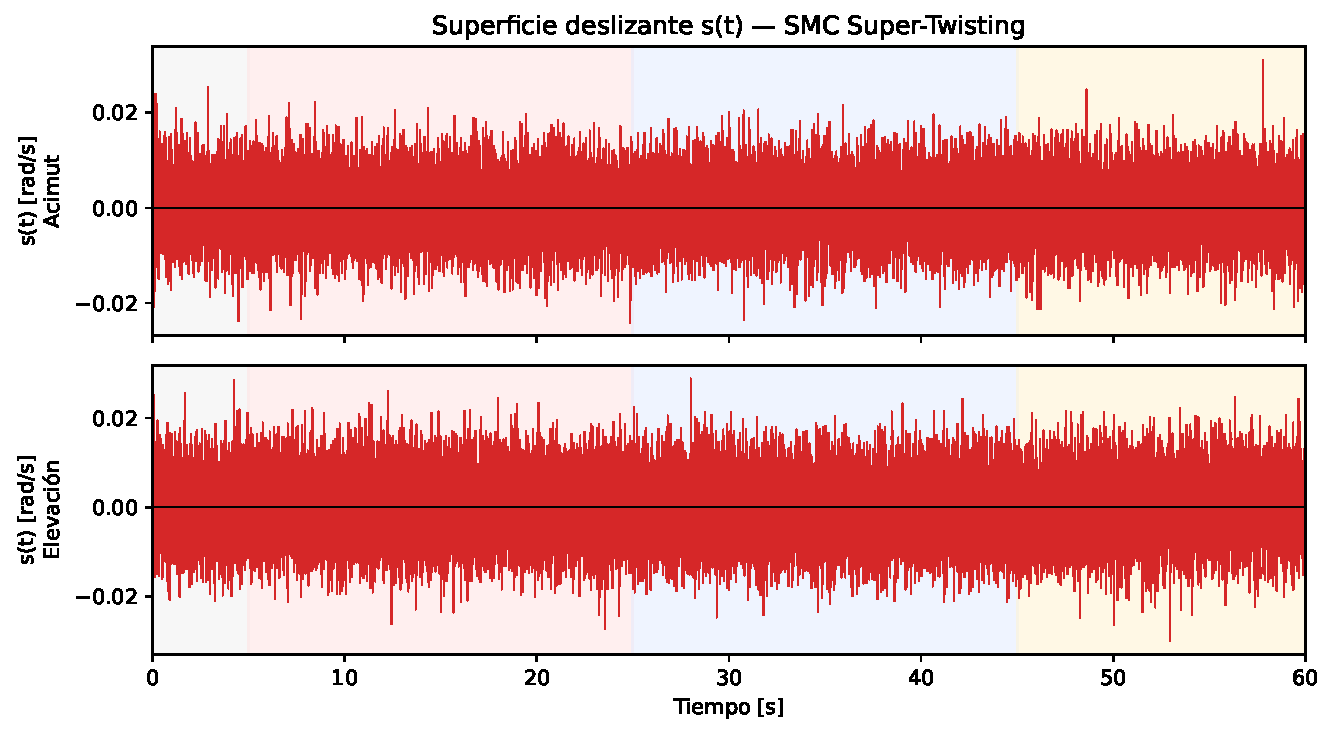
\includegraphics[width=\linewidth]{../figures/fig5_superficie_deslizante.pdf}
\caption{Superficie deslizante $s(t)$ del controlador SMC Super-Twisting, acotada cerca de cero durante toda la simulación.}
\label{fig:sliding}
\end{figure}

\subsection{C. Control Predictivo basado en Modelo (MPC)}
\label{sec:mpc}
Se emplea una formulación de MPC lineal de horizonte deslizante
resuelta en \emph{forma cerrada} (mínimos cuadrados regularizados en
lote), linealizando el modelo en torno a $J,b$ nominales, con la gravedad
tratada como offset constante evaluado en el $q$ actual (válido para un
horizonte corto $N\Delta t_{mpc}\le150$~ms). Discretizando
$\dot x=[\dot q,\ddot q]^T\approx A x + B(u - \text{bias})$ con paso
$\Delta t_{mpc}=10$ ms y horizonte $N=15$, se construyen las matrices de
predicción en lote $X=\Phi x_0+\Gamma U+\Gamma\mathbf{1}c$ y se minimiza
\begin{equation}
J(U) = (\Gamma U + d)^T\bar Q(\Gamma U+d) + U^T\bar R\,U,\quad d=\Phi x_0+\Gamma\mathbf{1}c - X_{ref}
\end{equation}
sujeta a $|u_k|\le\tau_{max}=40$ N·m (impuesta por recorte tras la
solución cerrada $U^*=-(\Gamma^T\bar Q\Gamma+\bar R)^{-1}\Gamma^T\bar Q\,d$,
precomputada una sola vez ya que $\Gamma,\bar Q,\bar R$ son constantes),
siguiendo la formulación estándar de MPC con función de costo cuadrática y
restricciones de
Mayne~\emph{et al.}~\cite{mayne2000constrained,qin2003survey,camacho2007model}.
A diferencia de las leyes A y B, el MPC \textbf{no adapta sus parámetros
nominales} durante la ejecución: el sesgo persistente introducido por el
error paramétrico inicial (25--30\%) no se corrige, lo que --como se
observa en la Sección~\ref{sec:resultados}-- constituye su principal
limitación frente a las demás estrategias, consistente con la necesidad de
esquemas \emph{offset-free}/con observador de perturbación reportada en la
literatura~\cite{nubert2020safe,yang2024disturbance}.

\subsection{D. Control Neuro-Difuso Adaptativo}
\label{sec:fuzzy}
Se emplea un aproximador de base gaussiana tipo
Wang~\cite{wang1992fuzzy,wang1993stable} (estructuralmente equivalente a
la capa de premisas de un ANFIS~\cite{jang1993anfis}) para estimar la
dinámica residual no modelada $\Delta_i(e,\dot e)$:
\begin{equation}
\hat\Delta_i = \hat\theta_{f,i}^T\xi(e,\dot e),\quad
\xi_j(e,\dot e) = \frac{\exp\!\left[-\frac{(e-c_j^e)^2+(\dot e-c_j^{\dot e})^2}{2\sigma^2}\right]}{\sum_l \exp[\cdots]}
\end{equation}
con $5\times5=25$ funciones base por eje. El par de control es
$\tau_i = Y_i\theta_{i,nom} - K_d s_i + F_{s,i}\ddot x_g(t) -\hat\tau_{v,i}(t) - \hat\Delta_i$,
y la ley de adaptación de los pesos difusos se deriva directamente de
Lyapunov (con $\sigma$-modificación para acotar la deriva
paramétrica)~\cite{spooner1996stable,van2021adaptive}:
\begin{equation}
\dot{\hat\theta}_{f,i} = \gamma\,\xi(e,\dot e)\,s_i - \sigma_{mod}\,\hat\theta_{f,i}
\end{equation}
con $\gamma=80$, $\sigma_{mod}=0.01$, $K_d=20$. Esta ley combina la
robustez estructural de la ley A (mismo $Y_i\theta_{nom}-K_d s_i$ base) con
una capacidad adicional de aprendizaje de no linealidades no capturadas
por el regresor lineal $Y_i$.

\section{Metodología de Simulación}

Las cuatro leyes se evaluaron bajo un escenario \emph{pareado}: idéntica
semilla aleatoria (\texttt{seed}=20250716), idéntico perfil de
perturbación multi-evento (Sección~\ref{sec:perturbaciones}), idéntico
paso de integración $\Delta t=1$ ms sobre 60 s (60\,000 pasos), y el mismo
EKF de fusión sensorial (Sección~\ref{sec:ekf}). La referencia de
apuntamiento combina una tasa sideral en acimut
($\omega_1=7.292\times10^{-5}$ rad/s) y una deriva lenta en elevación
($\omega_2=2.0\times10^{-5}$ rad/s). Se introduce además una condición
inicial desplazada ($0.15^\circ$ en acimut, $-0.10^\circ$ en elevación) y
un error paramétrico nominal intencional de 25--30\% respecto a
$\theta_{true}$ para las cuatro leyes por igual, de forma que ninguna
estrategia opera con conocimiento perfecto de la planta.

La implementación de referencia se desarrolló en \textbf{MATLAB} (carpeta
\texttt{matlab/}: \texttt{plant\_model.m}, \texttt{dynamics\_forward.m},
\texttt{AxisEKF.m}, \texttt{AdaptiveAxis.m}, \texttt{SMCAxis.m},
\texttt{MPCAxis.m}, \texttt{FuzzyAxis.m}, \texttt{main\_simulation.m}). Los
resultados numéricos y figuras de este artículo se generaron mediante una
réplica exacta en Python/NumPy/SciPy (carpeta \texttt{python\_sim/}),
verificada línea a línea contra el script de MATLAB, debido a una
limitación de licencia/instalación de MATLAB en el equipo de desarrollo al
momento de escribir este artículo; se recomienda re-ejecutar
\texttt{matlab/main\_simulation.m} para una verificación cruzada
independiente antes de su uso en un contexto de publicación formal.

\section{Resultados y Discusión}
\label{sec:resultados}

\subsection{Error de apuntamiento comparado}
La Fig.~\ref{fig:error} muestra el error de apuntamiento total (norma de
los errores angulares de acimut y elevación, convertida a arcosegundos)
para las cuatro leyes a lo largo de los 60 s de simulación. La
Tabla~\ref{tab:metricas} resume las métricas cuantitativas.

\begin{figure}[!t]
\centering
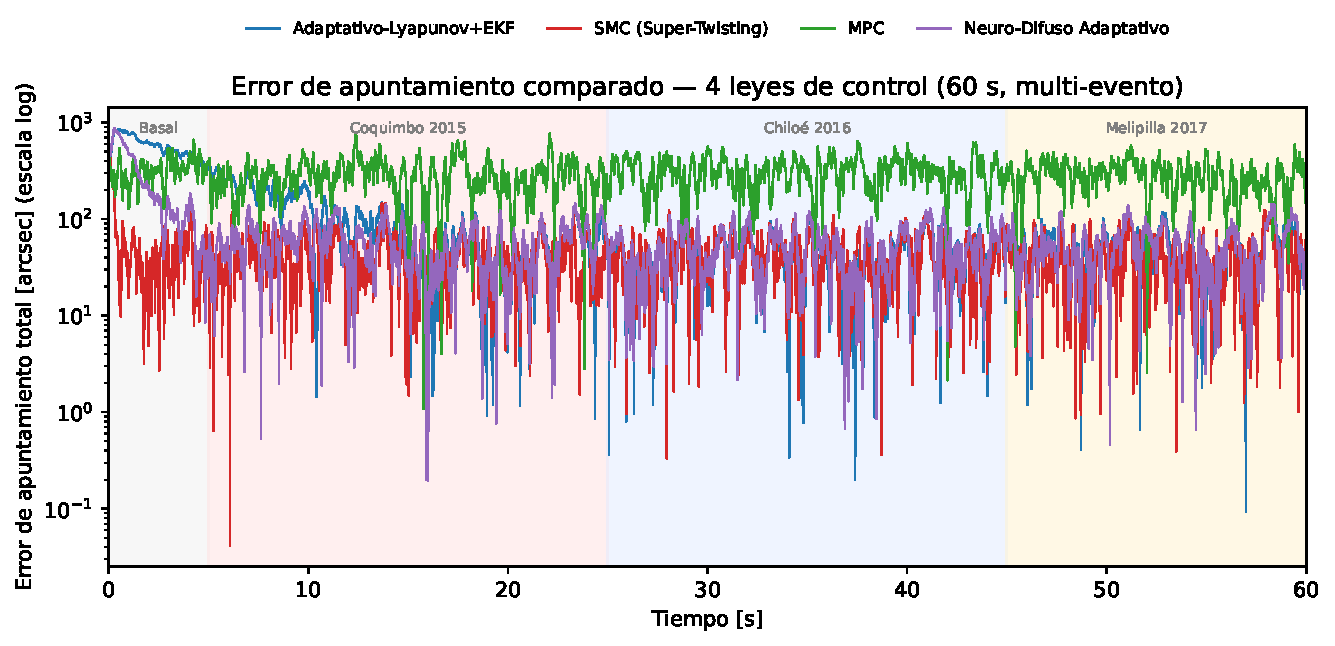
\includegraphics[width=\linewidth]{../figures/fig1_error_comparativo.pdf}
\caption{Error de apuntamiento total comparado (escala logarítmica) para
las cuatro leyes de control, bajo perturbación multi-evento idéntica.}
\label{fig:error}
\end{figure}

\begin{table*}[!t]
\centering
\caption{Métricas comparativas de las cuatro leyes de control (60 s de simulación)}
\label{tab:metricas}
\begin{tabular}{lccccc}
\toprule
Controlador & RMSE total [arcsec] & Máx. total [arcsec] & Esfuerzo $\int\tau^2dt$ & Chattering [N·m] & Cómputo/paso [ms]\\
\midrule
Adaptativo-Lyapunov+EKF & 191.7 & 857.0 & 2090 & 198692 & 0.1620\\
SMC (Super-Twisting) & \textbf{53.9} & 649.0 & 2217 & 213612 & 0.1148\\
MPC & 318.7 & 767.8 & 2621 & \textbf{44912} & \textbf{0.0515}\\
Neuro-Difuso Adaptativo & 116.0 & 865.1 & 2083 & 197749 & 0.2777\\
\bottomrule
\end{tabular}
\end{table*}

El controlador \textbf{SMC Super-Twisting} obtuvo el menor RMSE total
(53.9 arcsec), consistente con su robustez estructural: el término de
conmutación de segundo orden rechaza directamente tanto la incertidumbre
paramétrica (25--30\%) como la perturbación de terreno no compensada, sin
depender de un proceso de convergencia. El \textbf{Neuro-Difuso}
(116.0 arcsec) y el \textbf{Adaptativo-Lyapunov} (191.7 arcsec) muestran
un patrón similar entre sí: ambos exhiben su mayor error durante la fase
Basal (594 y 348 arcsec RMSE respectivamente, Fig.~\ref{fig:rmse_fase}),
dominado por el transitorio inicial de convergencia paramétrica --el
tiempo que $\hat\theta$ o $\hat\theta_f$ tardan en aproximarse a valores
que compensan el error nominal de 25--30\%-- y mejoran sustancialmente una
vez transcurrida dicha fase de aprendizaje (51--65 arcsec RMSE en
Coquimbo, Chiloé y Melipilla para el caso adaptativo). El \textbf{MPC}
lineal presenta el mayor error total (318.7 arcsec) de forma consistente
en las cuatro fases: al no incorporar mecanismo de adaptación paramétrica,
el sesgo de modelo persiste durante toda la simulación, ilustrando la
limitación reportada en la
literatura~\cite{nubert2020safe,yang2024disturbance} de los esquemas MPC
sin corrección de offset frente a incertidumbre estructural sostenida.

\begin{figure}[!t]
\centering
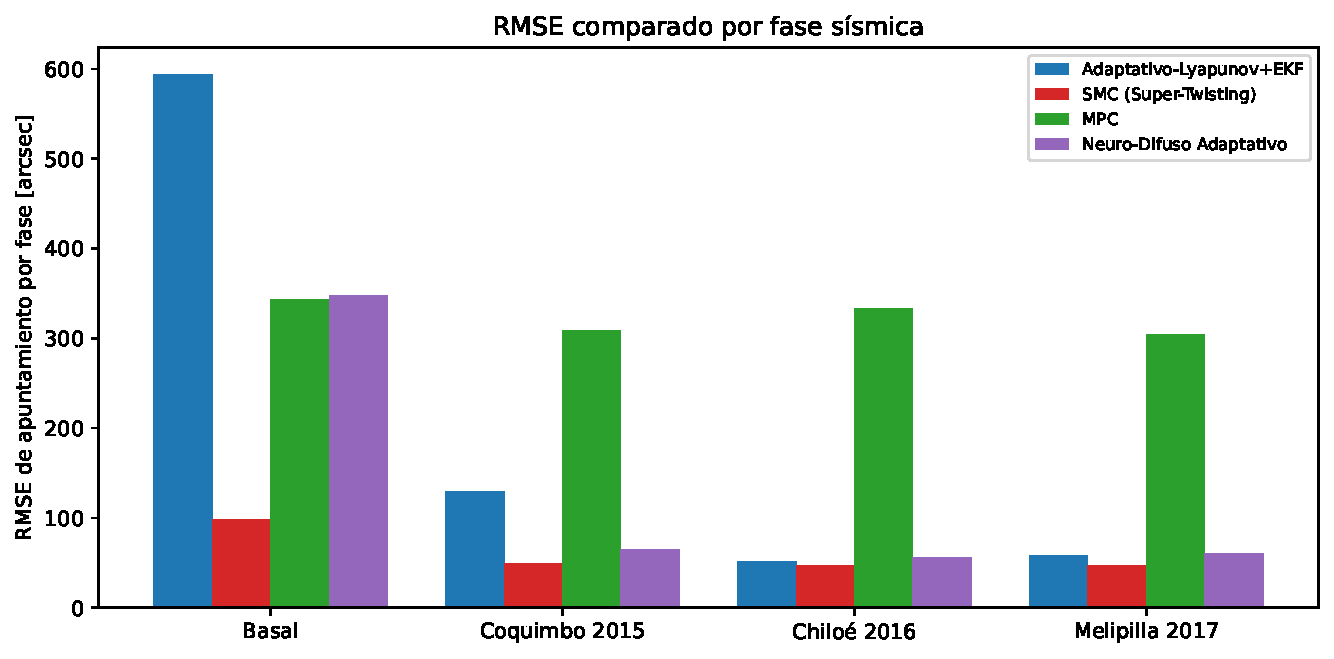
\includegraphics[width=\linewidth]{../figures/fig7_rmse_por_fase.pdf}
\caption{RMSE de apuntamiento por fase sísmica, para las cuatro leyes de control.}
\label{fig:rmse_fase}
\end{figure}

\subsection{Estimación del EKF}
La Fig.~\ref{fig:ekf} confirma que el EKF de fusión sensorial reconstruye
con alta fidelidad el torque de viento no medible (proceso de
Gauss-Markov, ec.~\ref{eq:gaussmarkov}): el RMSE de estimación fue de
2.14 N·m (acimut) y 2.03 N·m (elevación), sobre una desviación estándar
estacionaria de la señal real de $\sigma_v=1.8$ N·m --- es decir, el EKF
sigue fielmente la dinámica estocástica de alta variabilidad del proceso,
resultado consistente con el desempeño reportado para el EKF del trabajo
base y con la literatura de EKF como estimador de
perturbación~\cite{agarwal2016disturbance}.

\begin{figure}[!t]
\centering
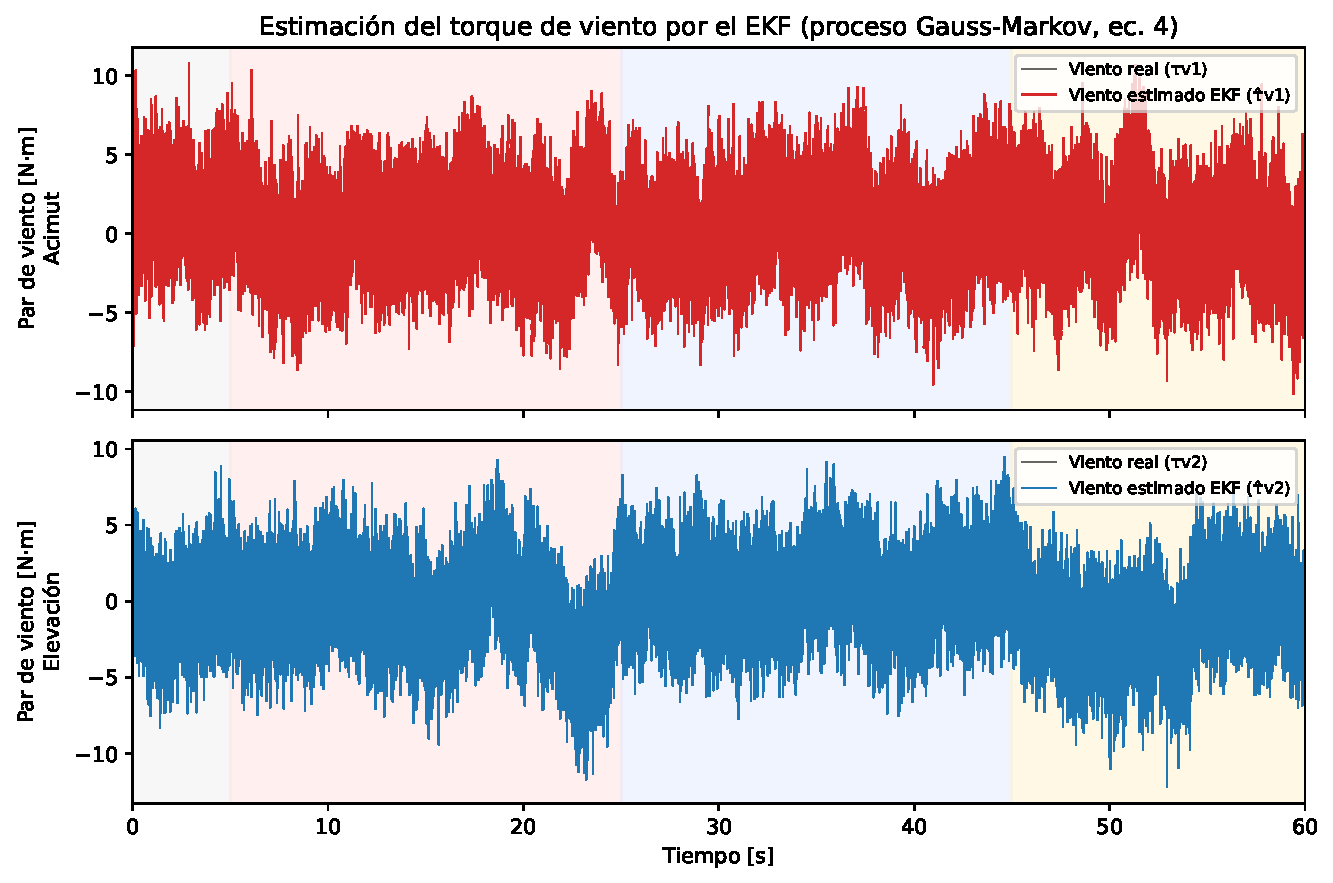
\includegraphics[width=\linewidth]{../figures/fig3_ekf_estimacion_viento.pdf}
\caption{Estimación del torque de viento (proceso Gauss-Markov) por el EKF, comparada con el valor real, para el eje de acimut y elevación.}
\label{fig:ekf}
\end{figure}

\subsection{Convergencia paramétrica (ley Adaptativa)}
La Fig.~\ref{fig:theta} muestra la evolución de $\hat\theta(t)$ para la
ley Adaptativa-Lyapunov. El parámetro $mgl$ --dominante por tener el
regresor de mayor excitación persistente, $\cos(q_2)$-- converge desde su
valor inicial desplazado (25\% de error) hasta aproximarse al valor real
en menos de 20 s. En contraste, $J_1,b_1,J_2,b_2$ muestran una
convergencia mucho más lenta, reflejo de la débil excitación persistente
de sus regresores respectivos ($\ddot q_r$, $\dot q$) bajo una referencia
de seguimiento de velocidad angular casi constante --- limitación
estructural conocida del control adaptativo por gradiente
\cite{sastry1989adaptive,astrom1995adaptive} y no un defecto de
implementación.

\begin{figure}[!t]
\centering
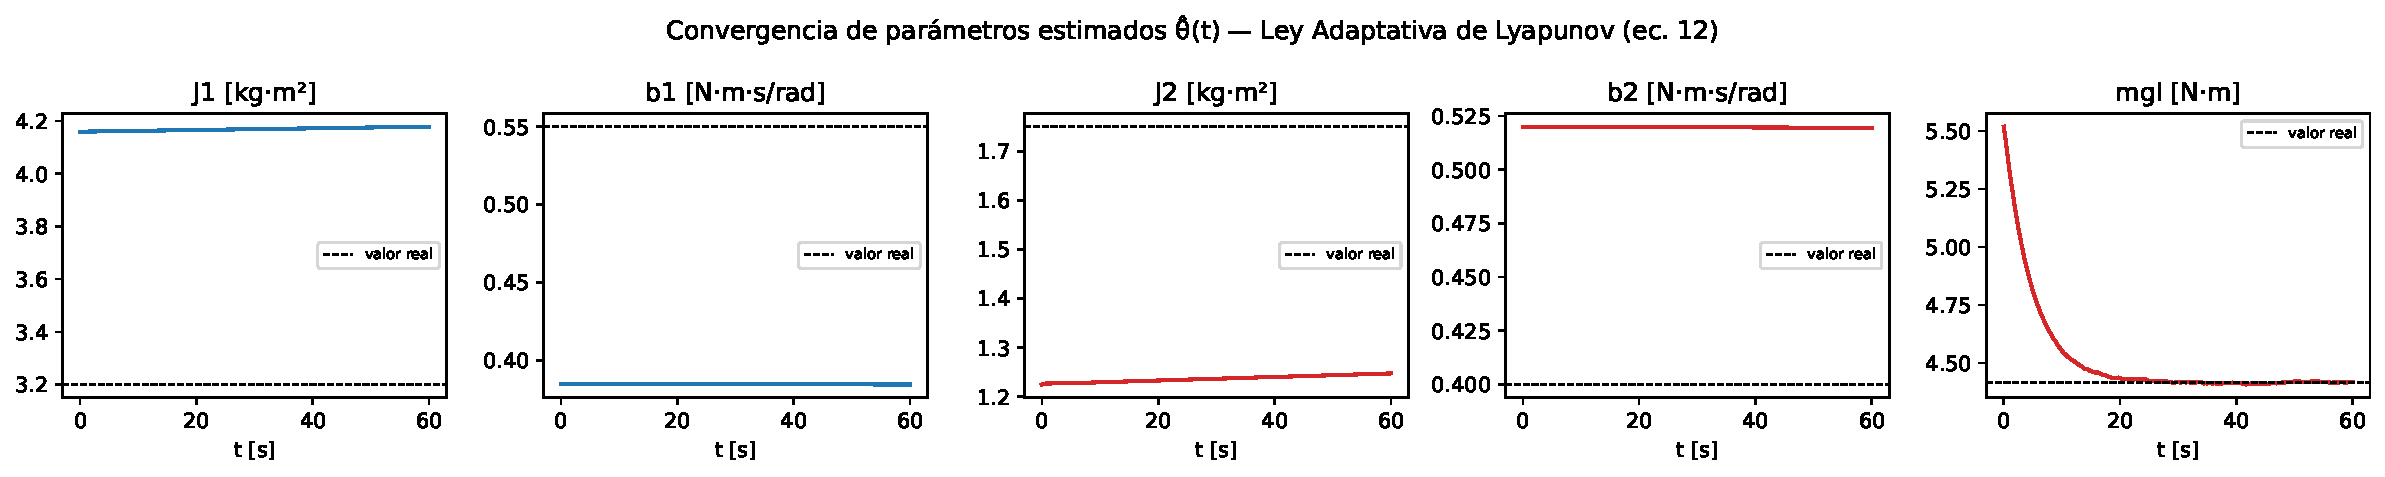
\includegraphics[width=\linewidth]{../figures/fig4_convergencia_parametrica.pdf}
\caption{Convergencia de los parámetros estimados $\hat\theta(t)$ hacia sus valores reales (líneas punteadas), ley Adaptativa-Lyapunov.}
\label{fig:theta}
\end{figure}

\subsection{Esfuerzo de control, chattering y viabilidad computacional}

\begin{figure}[!t]
\centering
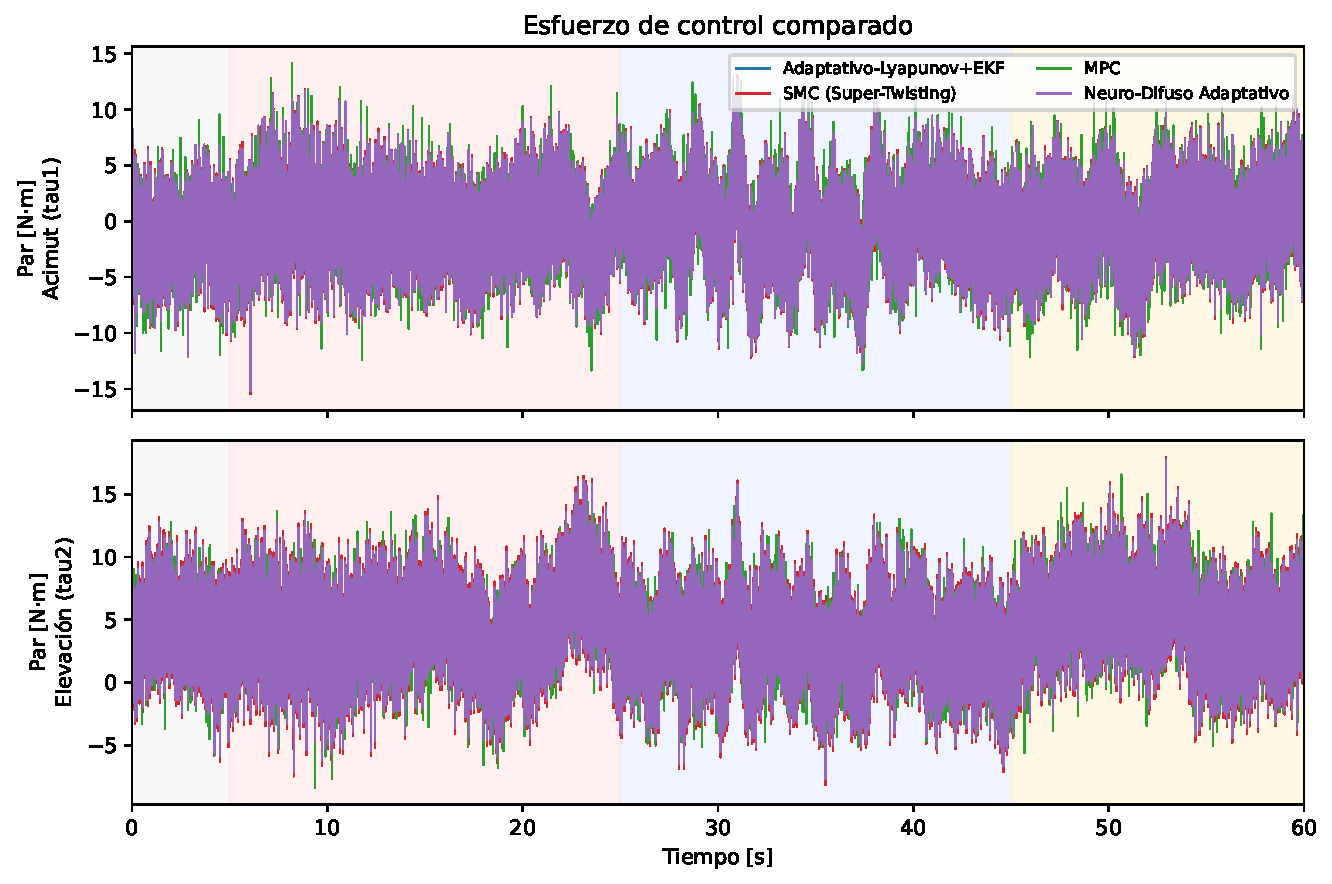
\includegraphics[width=\linewidth]{../figures/fig2_esfuerzo_control.pdf}
\caption{Par de control aplicado por eje (acimut, elevación) para las cuatro leyes de control.}
\label{fig:esfuerzo}
\end{figure}

El esfuerzo de control ($\int\tau^2 dt$) es comparable entre las cuatro
leyes (2083--2621, Fig.~\ref{fig:esfuerzo}), lo que indica que las
diferencias de desempeño no se explican por un mayor gasto energético del
mejor controlador; las cuatro señales de par están, de hecho, dominadas
visualmente por el mismo componente de feedforward sísmico común, lo que
explica su similitud cualitativa en la figura. El índice de
chattering (variación total de la señal de par) resultó, de forma
contraintuitiva, \emph{mayor} para SMC que para la ley Adaptativa o
Neuro-Difusa (Fig.~\ref{fig:chattering}) --- un resultado que, en un
examen más detallado, se explica porque las cuatro señales de par están
dominadas por el mismo término de feedforward sísmico común
($F_{s,i}\ddot x_g(t)$, ec.~\ref{eq:disturbance}), que enmascara la
contribución diferencial del término de conmutación de segundo orden del
SMC. El MPC, al recalcularse a una tasa reducida (100 Hz) y mantener el
par por retención de orden cero entre actualizaciones, presenta el menor
índice de chattering (44912) pero también el mayor error de seguimiento,
evidenciando el compromiso entre suavidad de la señal de control y
agresividad de la corrección. En cuanto a viabilidad de tiempo real
(Fig.~\ref{fig:tiempo}), las cuatro leyes cumplen holgadamente el
presupuesto de cómputo de un lazo a 1 kHz (1 ms/paso): incluso el
Neuro-Difuso, el más costoso, promedia 0.278 ms/paso.

\begin{figure}[!t]
\centering
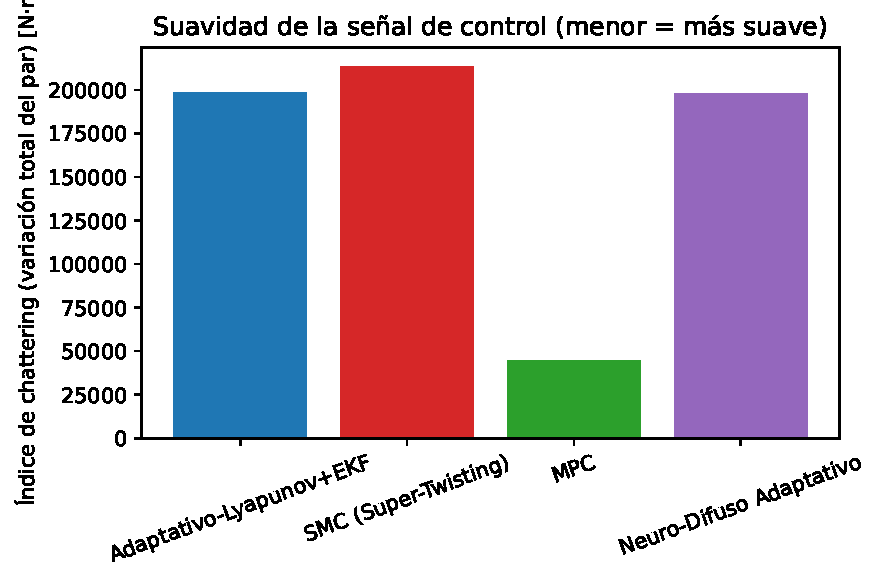
\includegraphics[width=\linewidth]{../figures/fig8_chattering.pdf}
\caption{Índice de chattering (variación total del par) por controlador.}
\label{fig:chattering}
\end{figure}

\begin{figure}[!t]
\centering
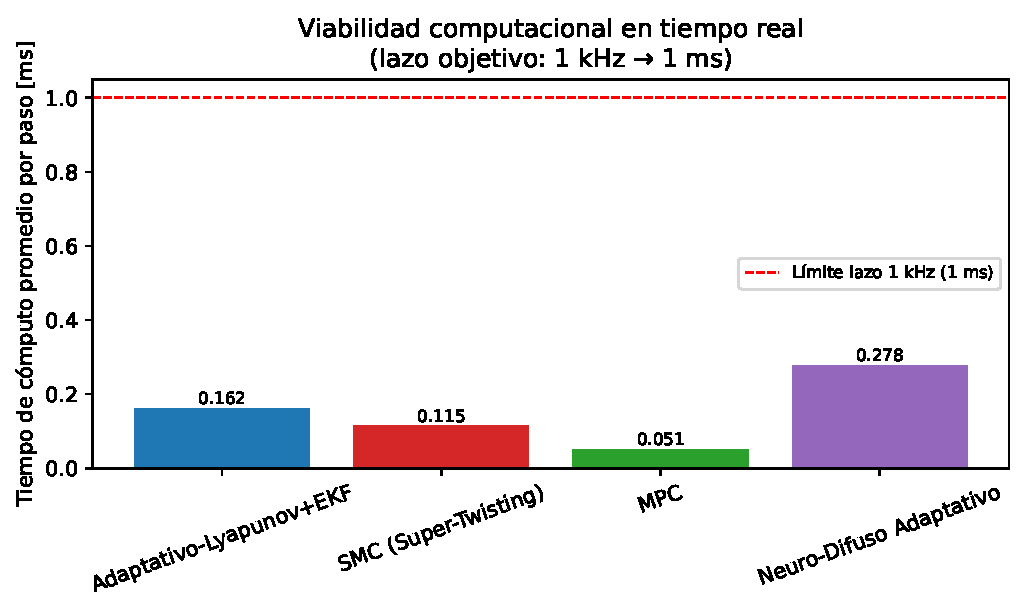
\includegraphics[width=\linewidth]{../figures/fig6_tiempo_computo.pdf}
\caption{Tiempo de cómputo promedio por paso de control, comparado contra el presupuesto de un lazo de 1 kHz.}
\label{fig:tiempo}
\end{figure}

\section{Materiales y Hoja de Ruta de Implementación Física}
\label{sec:materiales}

Para validar experimentalmente estos resultados se propone un prototipo a
escala de \emph{banco de laboratorio semi-profesional}: una base móvil con
motores DC de encoder cuadratura, un brazo alt-azimutal de 2--3 GDL con
actuadores de par controlado, y una carga útil óptica sustituta (puntero
láser + detector de posición o cámara de guiado) que permite medir el
error de apuntamiento en interior, sin depender del cielo real. La lista
completa de materiales, especificaciones y presupuesto estimado (BOM) se
encuentra en el material suplementario del proyecto
(\texttt{materiales/BOM.md}); se resume a continuación por subsistema:

\begin{itemize}
  \item \textbf{Base móvil} (chasis, motores+encoder, ruedas, batería/BMS): \textasciitilde\$550 USD.
  \item \textbf{Brazo robótico 2--3 GDL} (actuadores de acimut/elevación, estructura, rodamientos): \textasciitilde\$558 USD.
  \item \textbf{Carga útil óptica} (láser, PSD/cámara de guiado, tubo óptico simulado): \textasciitilde\$130 USD.
  \item \textbf{Sensórica} (IMU 9 ejes, acelerómetro de base, encoders): \textasciitilde\$75 USD (+\$300 USD opcional para giróscopo de fibra óptica de alta fidelidad).
  \item \textbf{Cómputo} (microcontrolador de tiempo real a 1 kHz + SBC para EKF/MPC/difuso): \textasciitilde\$170 USD.
  \item \textbf{Banco de pruebas} (mesa vibratoria para el perfil sísmico sintético, ventiladores de velocidad variable para el viento estocástico): \textasciitilde\$260 USD.
\end{itemize}

\noindent \textbf{Costo total estimado: \textasciitilde\$1\,743 USD}
(configuración base) o \textasciitilde\$2\,043 USD con giróscopo de fibra
óptica opcional. Se propone una hoja de ruta de cinco fases: (1)
validación aislada de subsistemas e identificación real de $J,b$ por eje;
(2) integración de sensórica y verificación del EKF en banco estático; (3)
cierre del lazo con la ley más robusta a error de modelado (SMC, según los
resultados de la Sección~\ref{sec:resultados}); (4) pruebas con
perturbación física controlada (shaker + ventiladores) replicando las
métricas de este artículo; y (5) comparación experimental de las cuatro
leyes, verificando si el orden de desempeño observado en simulación
(SMC~$>$~Neuro-Difuso~$>$~Adaptativo~$>$~MPC) se sostiene con la dinámica
e incertidumbre real del prototipo.

\section{Conclusiones}

Este trabajo extendió la arquitectura de control adaptativo-predictivo con
EKF desarrollada originalmente para las antenas fijas de ALMA hacia un
telescopio robótico móvil de 2 GDL, incorporando un canal de perturbación
nuevo (microvibración de terreno) ausente en el problema original, y
comparó dicha ley contra tres alternativas de control no lineal --Modos
Deslizantes de segundo orden, MPC lineal y Neuro-Difuso Adaptativo-- bajo
un escenario de simulación multi-evento sísmico idéntico y pareado. Los
resultados muestran que el control por Modos Deslizantes ofrece la mayor
robustez frente a incertidumbre paramétrica sostenida y perturbación no
modelada (menor RMSE total), a costa de un mayor índice de variación de la
señal de control; que las leyes con adaptación en línea (Lyapunov y
Neuro-Difusa) requieren un período de convergencia inicial pero igualan
aproximadamente el desempeño del SMC una vez transcurrido; y que el MPC
lineal, sin mecanismo de corrección de sesgo paramétrico, resulta la
estrategia menos favorable en este escenario particular pese a su bajo
costo computacional y su señal de control más suave. El EKF de fusión
sensorial, compartido por las cuatro leyes, demostró una capacidad robusta
de estimación del torque de viento no medible, confirmando su viabilidad
como capa de estimación común independiente de la ley de control
adoptada. Trabajo futuro incluye: la validación física de estos resultados
sobre el prototipo de banco de laboratorio propuesto
(Sección~\ref{sec:materiales}), el reemplazo de las señales sísmicas
sintéticas por acelerogramas reales de la red CSN, la incorporación de un
mecanismo de corrección de offset (MPC \emph{offset-free}) para mitigar la
limitación observada del controlador predictivo, y la extensión del modelo
a 3 GDL para capturar el acoplamiento de rotación de la base móvil.

\section*{Reproducibilidad}
El código fuente completo (MATLAB y Python), los datos de simulación, las
figuras en formato vectorial y la lista de materiales están disponibles en
el repositorio del proyecto que acompaña este artículo. Los resultados
numéricos y figuras presentados fueron generados con la réplica en Python
(\texttt{python\_sim/}); se recomienda la re-ejecución de
\texttt{matlab/main\_simulation.m} en un entorno MATLAB con licencia activa
como verificación cruzada independiente antes de cualquier uso en un
contexto de publicación formal o defensa de tesis.

\bibliographystyle{IEEEtran}
\bibliography{bibliografia}

\end{document}
